% ICASSP 2027 manuscript. The supplied Template.tex is intentionally preserved.
\documentclass{article}
\usepackage{spconf,amsmath,amssymb,amsthm,graphicx,booktabs,multirow}
\usepackage{tikz}
\usetikzlibrary{arrows.meta,positioning,calc,fit,backgrounds}
\usepackage{pgfplots}
\pgfplotsset{compat=1.18}
\usepackage{microtype,balance}
% \usepackage[hidelinks]{hyperref}
\usepackage{hyperref}
\usepackage{graphicx}
\usepackage{xcolor}
\newtheorem{proposition}{Proposition}
\newcommand{\Rpool}{R^2_{\mathrm{pool}}}
\newcommand{\Rbus}{R^2_{\mathrm{within}}}
\newcommand{\Sbus}{S_{\mathrm{bus}}}
\newcommand{\dP}{\Delta P}
\newcommand{\dQ}{\Delta Q}
\newcommand{\Vmag}{|V|}
\newcommand{\Pcal}{\mathcal{C}}
\newcommand{\Pproj}{\mathcal{P}}

\title{PHYSICS-INFORMED BUT NOT PHYSICS-CONSISTENT:\\
ERROR GEOMETRY AND SUBSPACE PROJECTION FOR NEURAL AC POWER FLOW}

\name{\begin{tabular}{c}
Changhun Kim$^{1}$, Timon Conrad$^{2}$, Redwanul Karim$^{1}$, Karan Pahlajani$^{1}$, Julian Oelhaf$^{1}$, David Riebesel$^{2}$\\
Tom\'as Arias-Vergara$^{1}$, Andreas Maier$^{1}$, Johann J\"ager$^{2}$, Siming Bayer$^{1}$
\end{tabular}%
\thanks{Corresponding author: changhun.kim@fau.de. This work was conducted within the scope of the research project GridAssist and was supported through the ``OptiNetD'' funding initiative by the German Federal Ministry for Economic Affairs and Energy (BMWE) as part of the 8th Energy Research Programme.}}
\address{$^{1}$Pattern Recognition Lab, Friedrich-Alexander-Universit\"at Erlangen-N\"urnberg, Germany\\
$^{2}$Institute of Electrical Energy Systems, Friedrich-Alexander-Universit\"at Erlangen-N\"urnberg, Germany}

\begin{document}
\ninept
\maketitle

\begin{abstract}
Recent neural power-flow solvers, including emerging foundation models,
achieve accurate voltage predictions, yet such accuracy does not
necessarily imply physically consistent solutions.
Even small voltage errors can yield large residuals from the AC power-balance.
We study this accuracy--consistency gap across PIGNN, GridSFM, gridfm-graphkit, and LUMINA on realistic 2224-bus GBnetwork scenarios, with cross-grid evaluation of GridSFM over 31 systems.
Using an SVD basis fitted to training AC power-flow solutions, we find that neural prediction errors contain substantial components outside the dominant solution subspace.
To address this mismatch,
calibrated solution-subspace projection (CSP) removes off-subspace prediction components,
substantially reducing mean power-balance residual from 0.3159 to 0.0550 p.u. for PIGNN-GC and
from 0.2687 to 0.0514 p.u. for GridSFM.
These results highlight output-error geometry as an important factor in physics-consistent neural AC power flow.
\end{abstract}







\begin{keywords}
AC power flow, neural surrogate, physics violation, error geometry, calibration, distribution shift
\end{keywords}

\section{Introduction}
\label{sec:introduction}

Modern power-system operation requires repeated AC power-flow (AC-PF) evaluations across increasingly diverse operating conditions driven by renewable generation, electrification, and changing demand \cite{decarne2024storage,conrad2025data}. AC-PF maps network conditions and power injections to bus voltages and flows serving as a fundamental nonlinear primitive in power-system analysis \cite{karimi2019loadflow}. Repeated evaluations arise in time-series and contingency studies \cite{oz2026dpf}, while the same AC network equations underlie optimization and state-estimation tasks \cite{monticelli2000state}.
%\begin{figure}[t]
%    \centering
%    \includegraphics[width=\columnwidth]
%    {Graphical_abstract.png}
%    \label{fig:graphical_abstract}
%    \caption{Neural AC-PF surrogates can achieve small voltage errors while retaining large physics violations. Bias calibration and solution-subspace projection jointly suppress systematic and off-subspace errors, improving both voltage accuracy and AC power-balance consistency.}
%\end{figure}
%\begin{figure}[t]
%    \centering
%    % Native TikZ version of the graphical abstract.  The Inkscape export is
%    % kept in Graphical_abstract.pdf_tex; to go back to it, replace the
%    % \resizebox line with
%    %   \def\svgwidth{\columnwidth}\input{Graphical_abstract.pdf_tex}
%    \resizebox{\columnwidth}{!}{\input{Graphical_abstract_tikz}}
%    \caption{Neural AC-PF surrogates can achieve small voltage errors while retaining large physics violations. Bias calibration and solution-subspace projection jointly suppress systematic and off-subspace errors, improving both voltage accuracy and AC power-balance consistency.}
%    \label{fig:graphical_abstract}
%\end{figure}

\begin{figure}[t]
    \centering
    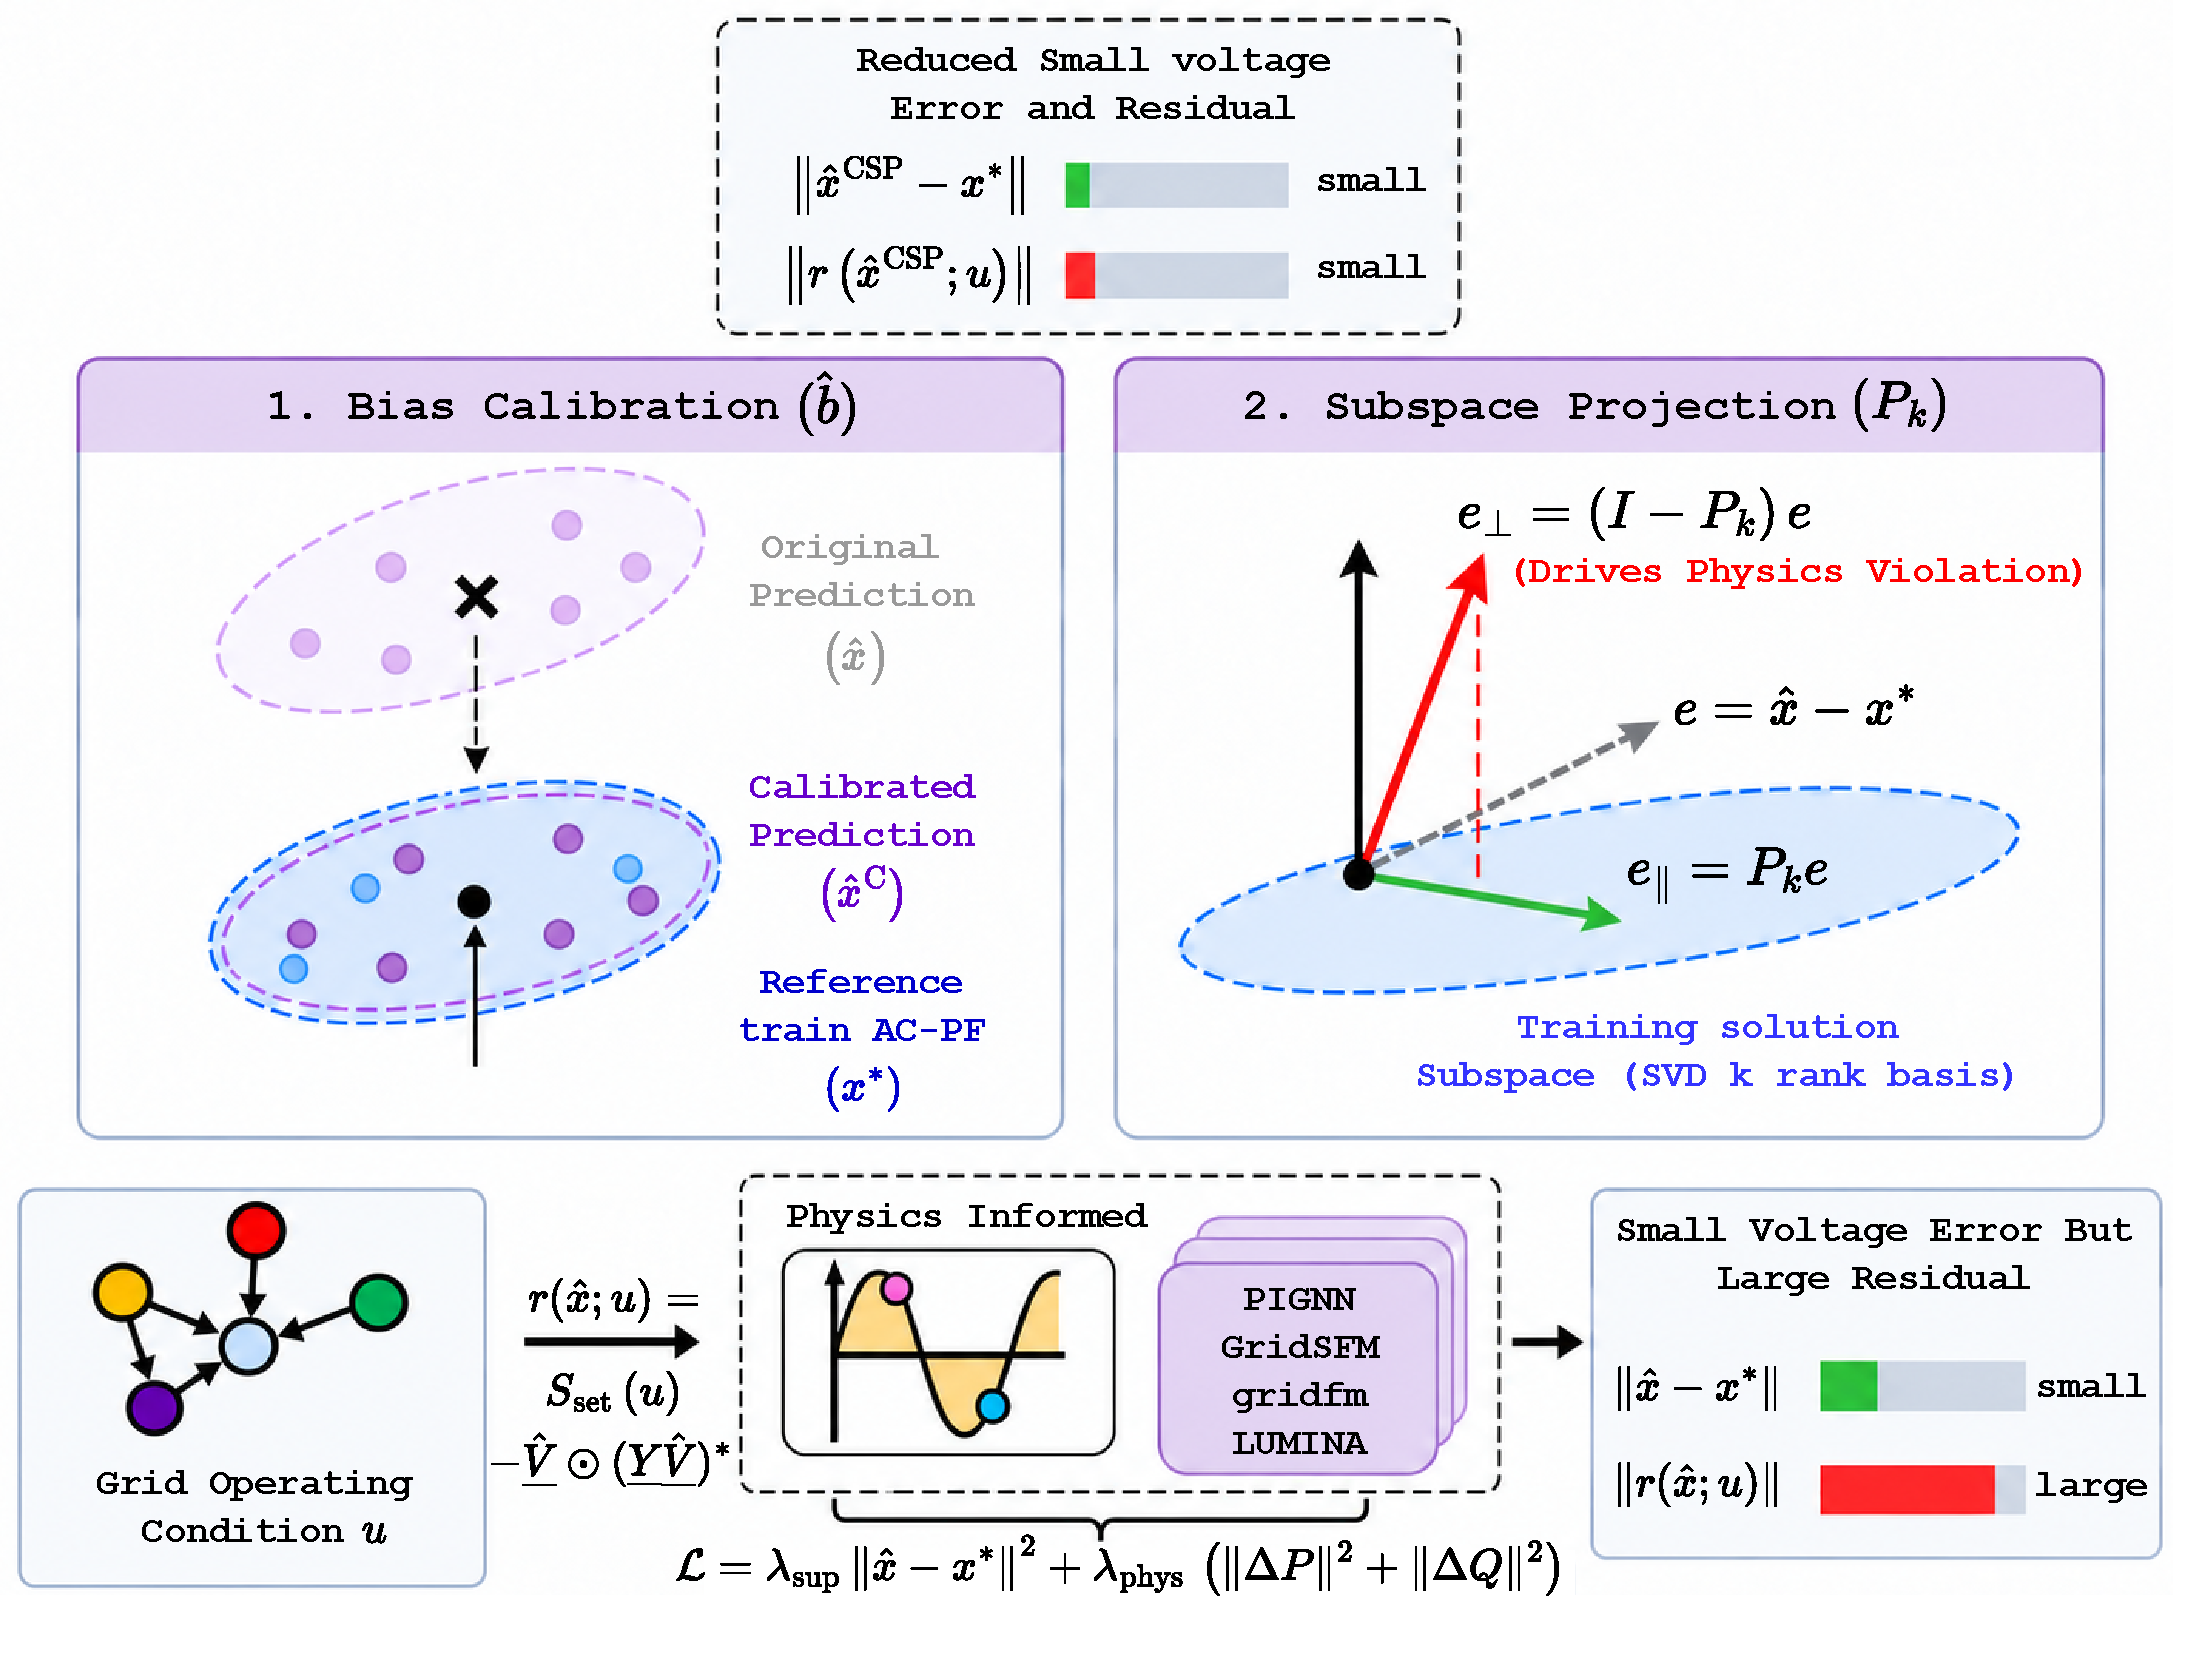
\includegraphics[width=\columnwidth]
    {csp_diagram_finished_x.pdf}
    \caption{Bias calibration and solution-subspace projection jointly suppress systematic and off-subspace errors, improving both voltage accuracy and AC power-balance consistency.}
    \label{fig:graphical_abstract}
\end{figure}

The computational demands of repeated grid analysis have motivated learned
surrogates that amortize the cost of conventional solvers over many operating
points \cite{lin2024powerflownet}.
Learned grid solvers span different levels of constraint enforcement:
direct regression prioritizes fast inference \cite{arowolo2026hhmpnn},
physics- or constraint-aware objectives penalize violations during training
\cite{piloto2024canos,wen2026pigat},
while iterative correction and feasibility-seeking mechanisms refine
predictions more directly toward physically consistent \cite{chzhen2026fab,pan2020deepopf} or feasible states
\cite{nguyen2025fsnet,donti2021dc3}.
More recent cross-grid and foundation-model efforts---including GridSFM
\cite{yang2026gridsfm}, gridfm-graphkit and GENCO
\cite{gridfmgraphkit2026,puech2026genco}, and LUMINA
\cite{li2026lumina}---extend this direction with global context and rich
heterogeneous, topology-aware representations designed to operate across
diverse grids and operating conditions.

Despite these advances, accurate voltage prediction does not necessarily imply
AC-consistent output \cite{ma2026safepowergraph}. Physics-informed objectives
can substantially reduce power-flow residuals
\cite{nellikkath2022pinn,ma2026safepowergraph}, but residual penalties remain
soft training objectives and do not by themselves enforce exact satisfaction
of the nonlinear AC equations. Consequently, small voltage-state errors can
coexist with non-negligible power-balance violations. This raises a question
not addressed by state accuracy alone: what properties of the remaining
voltage error determine how strongly it is translated into AC power-balance
residuals?

We hypothesize that the missing factor is the \emph{direction} of the remaining
voltage error: errors of similar magnitude may produce very different
power-balance residuals depending on how they are oriented across buses.
Goodwin et al. \cite{goodwin2026geometry} characterized the differential
geometry of the AC-PF solution manifold and assessed the quality of its linear
approximations. For neural surrogates, we instead study error geometry
empirically, asking whether the orientation of voltage errors relative to a
linear subspace estimated from training solutions helps explain the remaining
physical inconsistency.


We evaluate this hypothesis across PIGNN-GC, GridSFM, gridfm-graphkit, and LUMINA
on realistic 2224-bus GBnetwork scenarios, with additional cross-grid evaluation
of GridSFM over 31 systems of diverse sizes. Across all four models, train-only
calibration improves voltage accuracy while leaving persistent power-balance residuals, showing that persistent bias alone does not explain the
accuracy--consistency gap. We therefore construct an SVD basis exclusively from
training AC power-flow solutions and examine the orientation of the remaining
voltage errors relative to the resulting training-supported solution subspace.
Unlike Park et al., who use a PCA-based subspace to compress and reconstruct
AC-OPF outputs during learning \cite{park2024compact}, we use the
training-solution subspace to analyze surrogate-error geometry and to correct
frozen AC-PF predictions post hoc.

We find that substantial prediction error can lie outside the dominant
training-supported solution directions and that suppressing this off-subspace
component markedly reduces AC power-balance violations. Motivated by this
observation, we introduce \emph{calibrated solution-subspace projection} (CSP),
which first removes train-estimated bias and then suppresses prediction
components outside the dominant training-supported directions. CSP improves
voltage-magnitude accuracy and AC power balance simultaneously, while cross-grid
and distribution-shift experiments show that its benefits extend across diverse
systems but depend on how well the training-derived subspace represents the
operating distribution. Together, these results identify voltage-error geometry
across buses as an important link between state accuracy and physical
consistency.


Code: \href{http://github.com/Kimchangheon/neural-acpf-error-geometry}{github.com/Kimchangheon/neural-acpf-error-geometry}

\section{Error Geometry and Calibrated Subspace Projection}
\label{sec:method}

\subsection{AC power-balance consistency and train-only calibration}

We consider an $N$-bus grid with voltage state
$x=[V,\theta]\in\mathbb{R}^{2N}$, where
$\underline V=V\odot e^{\jmath\theta}$.
Given an operating condition $u$, a neural surrogate predicts
$\hat{x}=f_\phi(u)$, from which the AC active and reactive powers
$(P,Q)$ are recomputed using the network admittance model.
For setpoints $(P^{\mathrm{set}},Q^{\mathrm{set}})$, define
\[
r(\hat x;u)=
\begin{bmatrix}
\Delta P\\ \Delta Q
\end{bmatrix}
=
\begin{bmatrix}
P^{\mathrm{set}}-P\\
Q^{\mathrm{set}}-Q
\end{bmatrix},
\qquad
\mathrm{PB}=\sqrt{\Delta P^2+\Delta Q^2}.
\]
AC power-balance consistency is assessed by PB (Power Balance), evaluated bus-wise under the standard slack/PV/PQ conventions; Mean PB and Max PB are reported over buses and scenarios.
Before geometric analysis, we remove train-only post-training bias:
\[
\hat b=\mathbb{E}_{s\in\mathrm{tr}}[\hat x_s-x_s^\star],
\qquad
\hat x^C=\hat x-\hat b,
\]
with $\hat b$ frozen at test time. Angle offsets use circular differences
after gauge alignment; calibration removes bias without constraining
residual error directions.

\subsection{Error geometry in a training-derived solution subspace}

To characterize the remaining error, we construct a rank-$k$-per-channel basis
from Newton--Raphson solutions in the training set. Let $X_V$ and $X_\theta$
denote the centered training matrices of voltage magnitudes and gauge-aligned
angles, respectively. We compute separate SVDs
\begin{equation}
X_V=W_V\Sigma_VU_V^\top,\qquad
X_\theta=W_\theta\Sigma_\theta U_\theta^\top,\qquad
P_k=W_kW_k^\top,
\end{equation}
where $W_k=\operatorname{diag}(W_{V,k},W_{\theta,k})$ contains the leading
$k$ directions from each SVD; $k$ is capped by the available components on
smaller systems.

% \subsection{Error geometry in a training-derived solution subspace}
% To characterize the remaining error, we construct a rank-\(k\)-per-channel basis from Newton--Raphson solutions in the training set.
% Let $\bar x_{\mathrm{tr}}$ denote the training-solution mean and define
% \begin{equation}
% X=
% \begin{bmatrix}
% x_1^\star-\bar x_{\mathrm{tr}} & \cdots &
% x_{S_{\mathrm{tr}}}^\star-\bar x_{\mathrm{tr}}
% \end{bmatrix}
% =
% W\Sigma U^\top,\;
% P_k=W_kW_k^\top
% \end{equation}
% where $W_k=\operatorname{diag}(W_{V,k},W_{\theta,k})$ contains the leading
% $k$ SVD directions fitted separately to centered voltage magnitudes and
% gauge-aligned angles; $k$ applies to each channel and is capped by the
% available SVD components on smaller systems.
These subspaces capture dominant training-solution variation and define our error coordinates.
For $e=\hat x-x^\star$, we decompose
\begin{equation}
    e^{\parallel}=P_k e,
    \qquad
    e^{\perp}=(I-P_k)e ,
    \label{eq:error_decomposition}
\end{equation}
where $e^{\parallel}$ lies along the dominant training-solution directions
and $e^{\perp}$ captures error outside them.

%This decomposition is relevant to physical consistency because the AC
%residual is locally sensitive not only to the magnitude of the voltage
%error but also to its direction. Around a solved state $x^\star$,
%\begin{equation}
%    r(x^\star+e;u)
%    =
%    J(x^\star;u)e+\mathcal{O}(\|e\|^2),
%    \label{eq:local_residual}
%\end{equation}
%where $J$ is the AC residual Jacobian.
To relate this error decomposition to physical consistency, we use a
first-order Taylor expansion of the AC residual around a converged
power-flow solution $x^\star$:
\begin{equation}
    r(x^\star+e;u)
    =
    \underbrace{r(x^\star;u)}_{=0}
    +
    \underbrace{J(x^\star;u)e}_{\text{first-order term}}
    +
    \underbrace{\mathcal{O}(\|e\|^2)}_{\text{higher-order terms}},
    \label{eq:local_residual}
\end{equation}
where $J$ is the AC residual Jacobian.
Thus, the Jacobian determines how a given voltage error is translated
into power-balance residual: errors aligned with directions of larger
Jacobian gain can produce substantially larger residuals even when their
magnitudes are similar.
This motivates testing whether AC power balance changes when the voltage
error is rotated toward or away from the training-derived solution
subspace while its magnitude is held fixed.

\subsection{Calibrated solution-subspace projection (CSP)}

This motivates a direct intervention: suppress prediction components
outside the dominant training-solution directions while preserving the
variation supported by the data. Because systematic bias and off-subspace
error are distinct, we first apply post-training calibration and then
project the calibrated prediction:
\begin{equation}
    \boxed{
    \hat x^{\mathrm{CSP}}
    =
    \bar x_{\mathrm{tr}}
    +
    P_k
    \left(
        \hat x-\hat b-\bar x_{\mathrm{tr}}
    \right)
    }
    \label{eq:csp}
\end{equation}
where $\hat b$ is estimated from the trained model's predictions on the
training set and frozen at test time, while $\bar x_{\mathrm{tr}}$ and
$P_k$ are obtained solely from the training reference solutions.

The projection removes off-subspace prediction error, but can also discard
valid reference variation. To characterize this trade-off, let $e^C=\hat x^C-x^\star$. Since $P_k$ is orthogonal,
\begin{equation}
\|e^{\mathrm{CSP}}\|_2^2-\|e^C\|_2^2
=
\|(I-P_k)(x^\star-\bar x_{\mathrm{tr}})\|_2^2
-\|(I-P_k)e^C\|_2^2 .
\label{eq:tradeoff}
\end{equation}
Thus, CSP improves state accuracy when the removed off-subspace prediction
error exceeds the valid reference variation discarded by the projection.

CSP is a data-driven output correction rather than a projection onto the
nonlinear AC-feasible set, and therefore does not guarantee exact
satisfaction of the AC equations or operational constraints. Instead, it
tests whether suppressing off-subspace prediction components improves
voltage accuracy and recomputed AC power-balance residuals.

\section{Experiments and Results}
\label{sec:experiments}

\subsection{Experimental setup}
\label{sec:setup}

Our primary study uses 37,022 converged pandapower Newton--Raphson
operating points on the 2224-bus GBnetwork, split 1:1:1
for training/validation/test and varying load, generation, and PV setpoints~\cite{rivera2025pfdelta}.
We evaluate PIGNN-GC, our global-context extension of
PIGNN-Attn-LS~\cite{kim2026pignn}, GridSFM~\cite{yang2026gridsfm},
gridfm-graphkit v0.9.0~\cite{gridfmgraphkit2026}, and
LUMINA~\cite{li2026lumina}; GridSFM is additionally evaluated
cross-grid on 31 systems.

All models are trained from scratch using model-specific stable
initialization, and CSP is evaluated within each frozen model.
gridfm-graphkit uses its released architecture/configuration without a
pretrained checkpoint. GridSFM retains the released backbone but is adapted
from AC-OPF to AC-PF by fixing generator dispatch and training only for
voltage-state prediction with PF-specific residuals. LUMINA likewise retains
its released backbone but uses an enhanced AC-PF configuration with
known-variable masking, electrical bus features, and stabilized initialization.
For all models, electrical inputs, admittance, and evaluation use the same
pandapower internal PPC representation
\cite{thurner2018pandapower,zimmerman2011matpower}.



All calibration statistics and solution bases are fitted on training data
only. From $k\in\{4,8,16,32,64\}$, validation Mean PB selects
$k^\star=16$ without degrading calibrated voltage RMSE; this rank is then
frozen for all test and distribution-shift experiments.

Voltage RMSE alone can be small even when a model largely predicts a
static per-bus profile rather than following scenario-dependent voltage
variation~\cite{yang2026gridsfm}. To isolate this scenario-dependent
response, we center each bus as
$\tilde{V}_{is}=V_{is}-\bar{V}_i$ and
$\tilde{\hat{V}}_{is}=\hat{V}_{is}-\bar{\hat{V}}_i$, and report
\begin{equation}
R_{\mathrm{w}}^2
=
\operatorname{corr}^2
\left(\tilde{V}_{is},\tilde{\hat{V}}_{is}\right),
\qquad
a_{\mathrm{w}}
=
\frac{\operatorname{Cov}
\left(\tilde{V}_{is},\tilde{\hat{V}}_{is}\right)}
{\operatorname{Var}\left(\tilde{V}_{is}\right)} .
\end{equation}
$R_{\mathrm{w}}^2$ is the squared correlation between the centered
prediction and reference, while $a_{\mathrm{w}}$ measures the magnitude
of the predicted variation relative to the true variation.
% A per-bus constant predictor gives
% $R_{\mathrm{w}}^2=a_{\mathrm{w}}=0$ under our convention,
% while per-bus calibration leaves both metrics unchanged
% because the offset vanishes after centering.

\subsection{Fixed-norm directional intervention.}
We vary the orientation of the voltage-magnitude error relative to the
training-derived solution subspace while holding its $\ell_2$ norm fixed,
thereby isolating direction from error magnitude. Starting from the
calibrated prediction, we define
\begin{equation}
\tilde e(\alpha)
=
\|e_V\|_2
\frac{e_V^\parallel+\alpha e_V^\perp}
{\|e_V^\parallel+\alpha e_V^\perp\|_2}.
\label{eq:controlled_geometry}
\end{equation}
Decreasing $\alpha$ suppresses off-subspace error; the control analogously
suppresses the in-subspace component by exchanging
$e_V^\parallel$ and $e_V^\perp$. Phase angles are held fixed and Mean PB
is normalized at $\alpha=1$. Across all four surrogates, suppressing
off-subspace error consistently reduces Relative Mean PB, whereas
suppressing in-subspace error produces the opposite trend
(Fig.~\ref{fig:error_geometry}). Although the effect size varies across models, its direction is consistent.
Because the voltage-magnitude error norm is fixed throughout the intervention,
these results show that error orientation affects AC power-balance violation
independently of error magnitude.

Consistent with the fixed-norm experiment, a complementary local Jacobian
analysis shows that off-subspace perturbations produce larger AC-residual
changes per unit perturbation norm than in-subspace perturbations.
In a model-independent audit of 4,096 paired random directions at 128
held-out operating points, the median ratio of off- to in-subspace
Jacobian gain is $1{,}563\times$. The same directional sensitivity is
present in the actual calibrated prediction errors: the corresponding
off-/in-subspace gain ratios are $22.81\times$, $575.83\times$,
$4.69\times$, and $6.51\times$ for PIGNN-GC, GridSFM,
gridfm-graphkit, and LUMINA, respectively. The first-order expansion in
Eq.~\eqref{eq:local_residual} remains accurate in the observed error
regime, with median linearized-to-nonlinear residual-change ratios between
$0.996$ and $1.009$ across all four models.

% Consistent with the fixed-norm experiment, a complementary local Jacobian
% analysis shows that perturbations outside the training-solution subspace
% are far more strongly amplified into AC residuals than those inside it.
% Across 4,096 paired directions at 128 held-out points, median residual
% gain is 9.18 in-subspace versus 14,430 off-subspace ($1{,}560\times$).

% At 128 held-out operating points, we sample 32 random directions and
% compare the corresponding in- and off-subspace components, yielding
% 4,096 paired comparisons. The median residual gain is $9.18$ in-subspace
% and $14{,}430$ off-subspace, a difference of about $1{,}560\times$.

\begin{figure}[t]
    \centering
    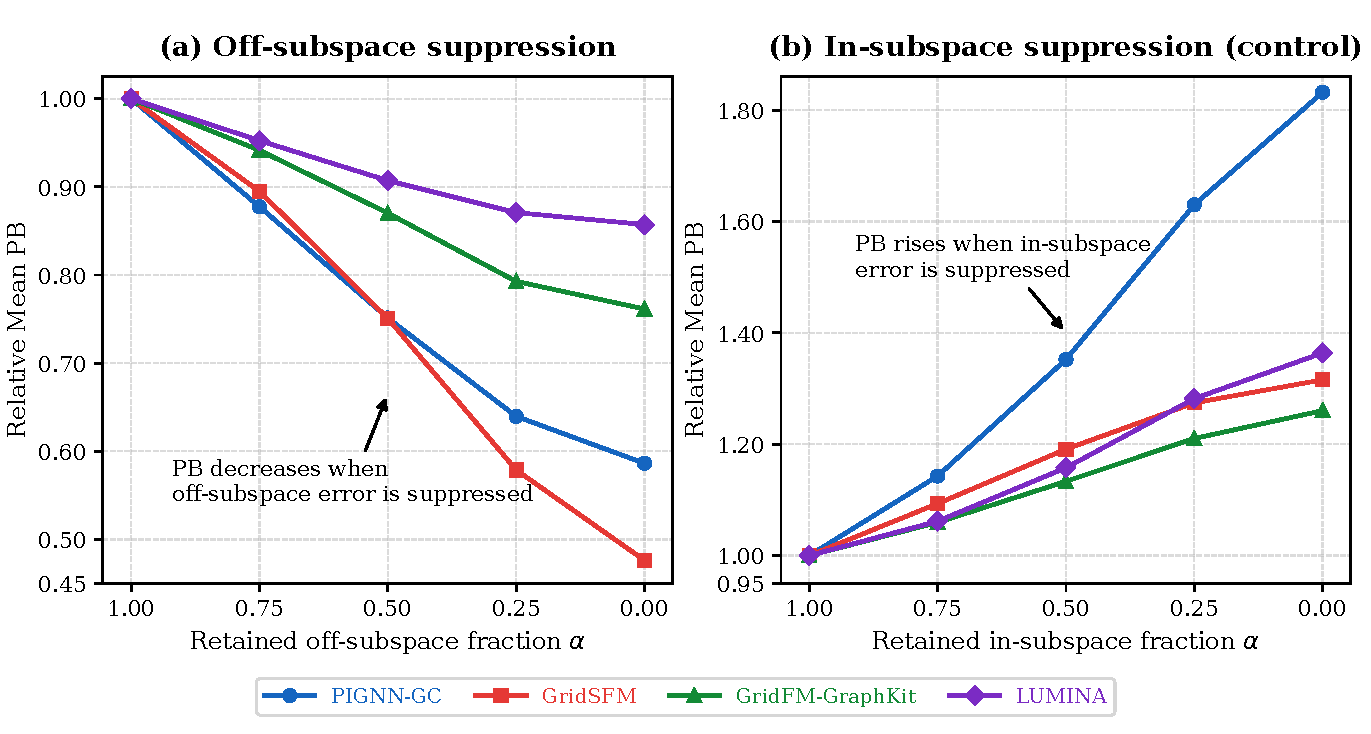
\includegraphics[width=\columnwidth]
    {figure1_controlled_error_geometry_updated.pdf}
    \caption{
    Fixed-norm directional intervention on GBnetwork, with Relative Mean PB
    normalized at $\alpha=1$.
    }
    \label{fig:error_geometry}
\end{figure}



\subsection{Specificity of the solution subspace.}
To test whether the observed benefit follows from generic dimensionality
reduction or graph smoothing, we replace the solution-SVD projection in
CSP with matched random, graph-Laplacian, and spatial low-pass projections.
As shown in Table~\ref{tab:basis_control}, only the training-solution SVD
improves both voltage-magnitude accuracy and power balance while increasing
$R_{\mathrm{w}}^2$ from $.685$ to $.853$ and nearly preserving
$a_{\mathrm{w}}$. In contrast, all three controls degrade scenario tracking
and substantially increase AC residuals. Thus, the CSP gain cannot be
explained by low dimensionality or spatial smoothing alone, but depends on
the orientation of the training-solution subspace.

% Matched random, Laplacian low-frequency, and spatial low-pass projections
% test whether CSP merely exploits dimensionality reduction or smoothing.
% Only the solution SVD improves $|V|$ accuracy and PB while raising
% $R_{\mathrm{w}}^2$ from $.685$ to $.853$ with nearly unchanged
% $a_{\mathrm{w}}$; all controls degrade tracking and residuals.
% Thus, the gain depends on basis orientation rather than low dimensionality
% or smoothing alone.

% To further rule out simple contraction toward the training mean, a
% validation-tuned isotropic shrinkage baseline selects $\lambda=1$, i.e.,
% no shrinkage, when calibrated voltage accuracy is preserved; stronger
% shrinkage reduces PB only at substantial cost to state accuracy and
% scenario-dependent variation.

\begin{table}[t]
\centering
\caption{
Basis controls on GBnetwork for PIGNN-GC (seed 42, $k=16$).
Random denotes the mean over eight independently sampled bases.
}
\label{tab:basis_control}
\setlength{\tabcolsep}{2.2pt}
\footnotesize
\resizebox{\columnwidth}{!}{
\begin{tabular}{lrrrrr}
\toprule
Projection &
$|V|$ RMSE $\downarrow$ &
Angle RMSE ($^\circ$) $\downarrow$ &
$R_{\mathrm{w}}^2 \uparrow$ &
$a_{\mathrm{w}}$ &
Mean PB $\downarrow$ \\
\midrule
None ($C$)
& .01421 & \textbf{.753} & .68522 & \textbf{.49329} & .14511 \\
Solution SVD
& \textbf{.01287} & .822 & \textbf{.85299} & .48903 & \textbf{.05690} \\
Random
& .02336 & 6.825 & .00540 & .00290 & 17.74 \\
Laplacian LF
& .02132 & 5.901 & .20128 & .12304 & 30.53 \\
Spatial LP
& .01568 & 1.926 & .63080 & .40717 & 29.29 \\
\bottomrule
\end{tabular}
}
\end{table}

% \subsection{Shrinkage control.}
% To test whether CSP simply benefits from contracting predictions toward
% the training mean, we consider
% \[
% \hat x^\lambda
% =
% \bar x_{\mathrm{tr}}
% +\lambda(\hat x^C-\bar x_{\mathrm{tr}}),
% \qquad 0\leq\lambda\leq1.
% \]
% We select $\lambda$ on the validation set by minimizing Mean PB subject
% to $|V|$ RMSE not exceeding that of calibration. The only admissible
% value is $\lambda^\star=1$, i.e., no shrinkage. Without this accuracy
% constraint, $\lambda=.125$ lowers Mean PB by 17.1\% but increases
% $|V|$ RMSE by 55.1\% and angle RMSE from $.734^\circ$ to $5.940^\circ$.
% Moreover, shrinkage leaves $R_{\mathrm{w}}^2$ nearly unchanged while
% reducing $a_{\mathrm{w}}$ approximately in proportion to $\lambda$.
% Thus, unlike CSP, scalar shrinkage trades prediction accuracy and
% response amplitude for lower residuals.

\subsection{Post-training CSP correction}

Table~\ref{tab:intervention} compares raw predictions, calibration ($C$),
projection ($P_{16}$), and CSP$_{16}$ on frozen outputs from PIGNN-GC,
GridSFM, gridfm-graphkit, and LUMINA. Relative to $C$, CSP reduces Mean
PB by $67.0\%$, $37.8\%$, $40.5\%$, and $71.1\%$, respectively, while
lowering voltage-magnitude RMSE in all four models. Projection also
increases $R_{\mathrm{w}}^2$ with little change in $a_{\mathrm{w}}$.
Angle accuracy is model dependent, degrading for the first three models
but improving for LUMINA. Raw and CSP$_{16}$ GPU inference times remain
comparable across all four models, indicating no discernible systematic
overhead from the post-training correction.

Comparing magnitude-only, angle-only, and full projection reveals that
the contribution of angle projection is model dependent. For PIGNN-GC,
full CSP gives the lowest PB among the projection variants, whereas
GridSFM achieves its lowest PB with magnitude-only projection.
For gridfm-graphkit, adding angle projection to the magnitude-only
correction reduces Mean/Max PB from $.0612/18.23$ to $.0457/5.08$,
but increases angle RMSE from $.367^\circ$ to $.496^\circ$.
For LUMINA, the same addition reduces Mean/Max PB from $.1939/38.53$
to $.0660/4.51$ while also improving angle RMSE from $1.374^\circ$
to $1.215^\circ$. Thus, improved physical consistency from angle projection does not
necessarily coincide with improved angle accuracy.

These model-dependent accuracy changes are explained by
Eq.~\eqref{eq:tradeoff}. For magnitude, the removed off-subspace
prediction-error energy exceeds the discarded reference variation
across all four models. For angle, the balance differs across models:
in gridfm-graphkit, angle projection discards more valid reference
variation than model error and therefore worsens angle RMSE, whereas
the opposite holds for LUMINA.
\begin{table*}[t]
\centering
\caption{
GBnetwork results at $k=16$.
PIGNN-GC, GridSFM, and gridfm-graphkit report mean $\pm$ standard
deviation over three model seeds; LUMINA is reported for seed 42.
$C$ denotes calibration, $P_{16}$ projection, and CSP$_{16}$ their
composition. Inference time is GPU-synchronized forward execution plus
the corresponding output transform, reported per scenario.
}
\label{tab:intervention}
\setlength{\tabcolsep}{3.5pt}
\resizebox{\textwidth}{!}{
\begin{tabular}{llrrrrrrr}
\toprule
Model & Output &
$|V|$ RMSE $\downarrow$ &
Angle RMSE ($^\circ$) $\downarrow$ &
$R_{\mathrm{w}}^2 \uparrow$ &
$a_{\mathrm{w}}$ &
Mean PB $\downarrow$ &
Max PB $\downarrow$ &
Inference (ms/scen.) \\
\midrule

Per-bus mean
& Baseline
& .02341
& 6.847
& .000
& .000
& .12084
& 5.88
& -- \\

\midrule
PIGNN-GC
& Raw
& $.02850 \pm .00232$
& $1.108 \pm .175$
& $.671 \pm .050$
& $.546 \pm .072$
& $.31592 \pm .03240$
& $195.89 \pm 52.54$
& $22.031 \pm .209$ \\

& $C$
& $.01393 \pm .00105$
& $\mathbf{.777 \pm .161}$
& $.671 \pm .050$
& $.546 \pm .072$
& $.16661 \pm .02352$
& $190.00 \pm 37.53$
& $22.045 \pm .255$ \\

& $P_{16}$
& $.01624 \pm .00254$
& $1.091 \pm .166$
& $.829 \pm .045$
& $.541 \pm .071$
& $.07594 \pm .00422$
& $5.07 \pm .85$
& $21.954 \pm .127$ \\

& CSP$_{16}$
& $\mathbf{.01222 \pm .00134}$
& $.835 \pm .141$
& $.829 \pm .045$
& $.541 \pm .071$
& $\mathbf{.05497 \pm .00257}$
& $\mathbf{3.93 \pm .07}$
& $22.046 \pm .206$ \\

\midrule
GridSFM
& Raw
& $.02868 \pm .01652$
& $2.294 \pm .302$
& $.768 \pm .151$
& $.724 \pm .149$
& $.26867 \pm .13004$
& $9.10 \pm 4.02$
& $25.045 \pm .207$ \\

& $C$
& $.01086 \pm .00403$
& $\mathbf{1.781 \pm .055}$
& $.768 \pm .151$
& $.724 \pm .149$
& $.08251 \pm .01093$
& $7.29 \pm 3.53$
& $25.015 \pm .096$ \\

& $P_{16}$
& $.01814 \pm .01145$
& $2.244 \pm .325$
& $.936 \pm .032$
& $.724 \pm .149$
& $.07630 \pm .01942$
& $5.08 \pm .49$
& $25.087 \pm .279$ \\

& CSP$_{16}$
& $\mathbf{.00782 \pm .00307}$
& $1.807 \pm .053$
& $.936 \pm .032$
& $.724 \pm .149$
& $\mathbf{.05136 \pm .00143}$
& $\mathbf{4.94 \pm .42}$
& $24.577 \pm .091$ \\

\midrule
gridfm-graphkit
& Raw
& $.00892 \pm .00154$
& $.385 \pm .042$
& $.905 \pm .030$
& $.811 \pm .045$
& $.09282 \pm .01763$
& $19.82 \pm 8.65$
& $5.917 \pm .019$ \\

& $C$
& $.00753 \pm .00118$
& $\mathbf{.367 \pm .042}$
& $.905 \pm .030$
& $.811 \pm .045$
& $.07685 \pm .01307$
& $18.88 \pm 8.69$
& $5.730 \pm .004$ \\

& $P_{16}$
& $.00617 \pm .00099$
& $.503 \pm .018$
& $\mathbf{.959 \pm .008}$
& $.801 \pm .044$
& $.04593 \pm .00156$
& $5.36 \pm .56$
& $5.723 \pm .011$ \\

& CSP$_{16}$
& $\mathbf{.00606 \pm .00090}$
& $.496 \pm .021$
& $\mathbf{.959 \pm .008}$
& $.801 \pm .044$
& $\mathbf{.04571 \pm .00135}$
& $\mathbf{5.08 \pm .18}$
& $5.779 \pm .012$ \\

\midrule
LUMINA
& Raw
& $.02689$
& $2.347$
& $.448$
& $.358$
& $.83072$
& $464.63$
& $8.469$ \\

& $C$
& $.01768$
& $1.373$
& $.448$
& $.358$
& $.22800$
& $38.85$
& $8.791$ \\

& $P_{16}$
& $.01943$
& $1.856$
& $\mathbf{.892}$
& $.350$
& $.07713$
& $4.83$
& $8.121$ \\

& CSP$_{16}$
& $\mathbf{.01549}$
& $\mathbf{1.215}$
& $\mathbf{.892}$
& $.350$
& $\mathbf{.06597}$
& $\mathbf{4.51}$
& $8.739$ \\

\bottomrule
\end{tabular}
}
\end{table*}

\subsection{Complementarity with one-step Newton refinement.}
We next test whether CSP remains useful when followed by an explicit
residual-directed correction. Starting from either calibrated outputs
($C$) or CSP$_{16}$, we apply exactly one Newton update
($\mathrm{NR}_1$), updating non-slack angles and PQ voltage magnitudes.
The damping factor is selected on validation data from
$\{0.25,0.5,0.75,1.0\}$ and fixed to $\eta=1$ for all models.
No Newton solve failures or damping fallbacks occur.

A single Newton step substantially improves both voltage accuracy and
power balance from either initialization. Importantly, the benefit of
CSP persists after this strong correction: relative to
$C+\mathrm{NR}_1$, CSP$_{16}+\mathrm{NR}_1$ reduces Mean PB by
$47.9\%$, $51.2\%$, $21.1\%$, and $81.0\%$ for PIGNN-GC, GridSFM,
gridfm-graphkit, and LUMINA, respectively, while also lowering
magnitude and angle errors in all four models. Thus, CSP and Newton
refinement address complementary aspects of the prediction error:
CSP provides a data-derived geometric correction, whereas
$\mathrm{NR}_1$ explicitly uses the AC Jacobian to reduce the remaining
residual.

The computational costs are correspondingly different. CSP requires
approximately two seconds for the full 12,344-scenario test set,
whereas one scenario-wise Newton correction requires approximately
$2.4$--$3.8\times10^3$\,s in our multiprocessing implementation.
These implementation-specific timings exclude neural inference and are
not hardware-normalized. CSP is therefore not a replacement for Newton
refinement, but a lightweight correction that also provides a better
initialization for a subsequent residual-directed update.

\begin{table*}[t]
\centering
\caption{
One Newton update from calibrated or CSP$_{16}$ outputs on GBnetwork.
Validation selects $\eta=1$ for all models.
}
\label{tab:nr1}
\setlength{\tabcolsep}{3.2pt}
\footnotesize
\resizebox{\textwidth}{!}{
\begin{tabular}{llrrrrrr}
\toprule
Model & Start &
$|V|$ RMSE $\downarrow$ &
Angle RMSE ($^\circ$) $\downarrow$ &
$R_{\mathrm{w}}^2 \uparrow$ &
$a_{\mathrm{w}}$ &
Mean PB $\downarrow$ &
Max PB $\downarrow$ \\
\midrule

PIGNN-GC
& $C$
& $.00180\pm.00012$
& $.119\pm.013$
& $.99705\pm.00030$
& $.975\pm.001$
& $.00284\pm.00046$
& $1.72\pm.82$ \\
& CSP$_{16}$
& $\mathbf{.00117\pm.00010}$
& $\mathbf{.073\pm.009}$
& $\mathbf{.99875\pm.00021}$
& $\mathbf{.979\pm.002}$
& $\mathbf{.00148\pm.00013}$
& $\mathbf{.782\pm.021}$ \\
\midrule
GridSFM
& $C$
& $.01186\pm.00677$
& $.681\pm.380$
& $.95000\pm.02347$
& $1.385\pm.266$
& $.00250\pm.00154$
& $.860\pm.255$ \\
& CSP$_{16}$
& $\mathbf{.00097\pm.00020}$
& $\mathbf{.059\pm.013}$
& $\mathbf{.99912\pm.00038}$
& $\mathbf{.983\pm.003}$
& $\mathbf{.00122\pm.00029}$
& $\mathbf{.848\pm.093}$ \\

\midrule
gridfm-graphkit
& $C$
& $.000943\pm.000232$
& $.0843\pm.0236$
& $.99922\pm.00037$
& $.98910\pm.00208$
& $.000941\pm.000325$
& $1.112\pm.549$ \\
& CSP$_{16}$
& $\mathbf{.000496\pm.000085}$
& $\mathbf{.0277\pm.0041}$
& $\mathbf{.99980\pm.00008}$
& $\mathbf{.99033\pm.00126}$
& $\mathbf{.000742\pm.000080}$
& $\mathbf{.624\pm.080}$ \\

\midrule
LUMINA
& $C$
& $.008687$
& $.6287$
& $.93290$
& $.93327$
& $.008936$
& $2.474$ \\
& CSP$_{16}$
& $\mathbf{.001057}$
& $\mathbf{.0838}$
& $\mathbf{.99910}$
& $\mathbf{.98270}$
& $\mathbf{.001694}$
& $\mathbf{.721}$ \\

\bottomrule
\end{tabular}
}
\end{table*}
\subsection{Cross-grid breadth and distribution shift}
\label{sec:breadth_shift}
\noindent\textit{Cross-grid breadth.}
Fig.~\ref{fig:crossgrid_csp} evaluates GridSFM with CSP across 31 systems
spanning 4--9,241 buses and sub-kV to 750-kV levels: 28
pandapower/PYPOWER-format systems from IEEE, PEGASE, RTE, and GB benchmark
families, plus three Common Information Model (CIM)-based networks.
For each system, calibration and subspace statistics are fitted from its
training data, using nominal $k=16$ per channel and the available SVD
components on smaller systems. CSP reduces GridSFM Mean PB across all
31 systems.

\begin{figure}[t]
    \centering
    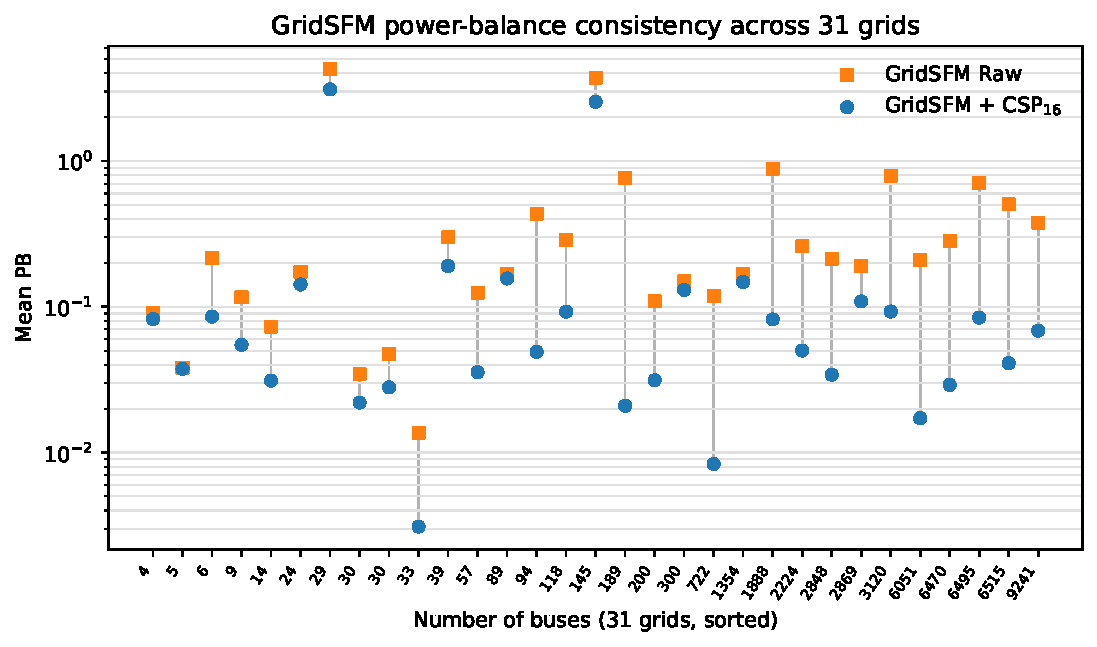
\includegraphics[width=\columnwidth]
    {gridsfm_raw_vs_csp16_discrete3.pdf}
    \caption{
    Grid-by-grid physical consistency of GridSFM before and after
    CSP$_{16}$ across 31 systems ordered by bus count. Mean PB is shown
    on a logarithmic scale.
    }
    \label{fig:crossgrid_csp}
\end{figure}

\vspace{0.35em}

\noindent\textit{Topology and spatial shifts.}
Under $N$--1/$N$--2 outages, tracking and bulk PB remain close to control,
with larger maxima indicating isolated topology-induced violations and the
need for worst-case assessment beyond average error
\cite{chevalier2022guarantees}.
GBcorr causes a broader shift: transferring both control calibration and
basis gives Mean PB $\approx0.100$ p.u. Refitting calibration alone reduces
this to $0.0944$, basis alone to $0.0740$, and both to $\approx0.068$.
The transferred basis retains $93.55\%$ of GBcorr magnitude variation,
versus $98.53\%$ after refitting, while reference-state projection reduces
Mean PB from $0.0868$ to $0.0438$ p.u. This shows that GBcorr introduces
not only calibration drift but also solution-subspace mismatch.

% We evaluate two distribution shifts with fixed model weights and nominal rank:
% $N$--1/$N$--2 line outages using the unchanged control calibration and
% subspace statistics, and GBcorr, which spatially redistributes load across
% 14 fixed synthetic connected zones using a covariance estimated from measured
% GB zonal demand while preserving total load and generation settings.
% For GBcorr, we additionally test joint condition-matched recalibration and
% subspace refitting on shifted training data.

% Topology shifts leave tracking and the bulk PB distribution close
% to control, but introduce substantially larger far-tail violations.
% GBcorr causes a broader degradation in tracking and PB; joint refitting reduces PB but only partially restores tracking, suggesting that further surrogate adaptation may be needed.

\begin{table}[t]
\centering
\caption{
Fixed-rank CSP$_{16}$ under topology and operating-distribution shifts.
T transfers the control-derived calibration and solution basis, whereas R
refits both on condition-matched training data. PB statistics are pooled
over all bus--scenario pairs.
}
\label{tab:shift}
\setlength{\tabcolsep}{1.8pt}
\footnotesize
\begin{tabular}{lrrrrrrrr}
\toprule
Condition &
RMSE$_V$ &
$R_{\mathrm{w}}^2 \uparrow$ &
$a_{\mathrm{w}}$ &
Mean &
Median &
p95 &
p99 &
Max \\
\midrule
Control
& .01281
& .8476
& .4866
& .0581
& .0131
& .2665
& .5462
& 3.58 \\
\midrule
$N$--1 (T)
& .01314
& .8391
& .4750
& .0603
& .0131
& .2713
& .5632
& 33.16 \\
$N$--2 (T)
& .01288
& .8458
& .4870
& .0617
& .0132
& .2713
& .5721
& 27.45 \\
\midrule
GBcorr (T)
& .01966
& .4819
& .4025
& .1003
& .0231
& .4512
& .9746
& 7.00 \\
GBcorr (R)
& \textbf{.01620}
& .5150
& .4247
& \textbf{.0680}
& .0174
& .3031
& \textbf{.6415}
& \textbf{4.99} \\
\bottomrule
\end{tabular}

% \vspace{0.2em}
% \parbox{\columnwidth}{\scriptsize
% T: transfer of the control basis; R: basis refitted using shifted
% training solutions only.}
\end{table}

\section{CONCLUSION}

This work identifies output-error geometry as an important factor in the
accuracy--consistency gap of neural AC-PF surrogates. Fixed-norm and
Jacobian analyses reveal strong directional sensitivity of AC residuals,
while CSP reduces power-balance residuals and improves voltage-magnitude
accuracy on GBnetwork. CSP also improves voltage accuracy and mean power-balance residuals after one Newton update, supporting its complementary role in
residual-directed refinement. Cross-grid evaluation shows that the power-balance
improvement extends beyond GBnetwork, whereas distribution-shift experiments
show that a fixed solution subspace can become mismatched to the shifted
operating distribution. These results motivate extending physics-consistent
neural surrogates toward broader power-system analysis, estimation, and
optimization.



\bibliographystyle{IEEEbib}
\bibliography{neural_pf_tracking_calibration_error_geometry}


\end{document}
